\def\pathToRoot{.}
\documentclass[a4paper, 12pt]{article}

\usepackage[utf8]{inputenc}
\usepackage{ifthen}
\usepackage{xparse}
\usepackage{scrextend}
\usepackage{setspace}
\usepackage{verbatim}
\usepackage{color}
\usepackage[inline]{enumitem}
\usepackage[colorlinks=true, linkcolor=black, citecolor=black]{hyperref}

\usepackage{tikz}
\usepackage{pgfplots}
\usepackage{bbold}
\usepackage{listings}

\usepackage{subcaption}

\usepackage{amsmath}
\usepackage{amssymb}
\usepackage{latexsym}
\usepackage{hyperref}
\usepackage{cleveref}

\definecolor{gray}{rgb}{0.2,0.2,0.2}

\pagenumbering{arabic}


\usepackage[a4paper, left=2cm, top=2cm, right=2cm, bottom=2cm]{geometry}

\usepackage{multirow}
\usepackage{fancyvrb}

\newcommand{\vect}[1]{\boldsymbol{#1}}

\newcounter{exerciseCounter}
\setcounter{exerciseCounter}{0}

\newcommand{\exerciseNumber}{\sheetnumber.\arabic{exerciseCounter}}

\setenumerate{label=\alph*)}

% Sheet Header
\newcommand{\exercisehead}[3]
{
    \def\sheetnumber{#1}
    \begin{center}
        \begin{minipage}{0.45\linewidth}
            \textsc{Universität des Saarlandes}
            \par
           Prof. Dr. Dietrich  Klakow
           \par
           Lehrstuhl für Signalverarbeitung
           \par
           NNIA Winter Term 2019/2020
        \end{minipage}
        \begin{minipage}{0.45\linewidth}
            \begin{flushright}
               
\includegraphics[width=0.30\linewidth]{headers/lsv_logo.jpg}
            \end{flushright}
        \end{minipage}
        \vspace{5pt}
        \hrule
        \vspace{12pt}
        \doublespacing
        {
            \LARGE
            \textbf{Exercise Sheet #1}
        }
        \par
        {
            \large
            #2
        }
        \par
        \ifdefined\issolution
        \textit{(Solutions)}
        \else
        \fi
        
    \textbf{Deadline: #3}

    \end{center}
    \vspace{2pt}
    \hrule
    \vspace{12pt}
}

% Exercise environment
\NewDocumentEnvironment{exercise}{oo}
{
	\refstepcounter{exerciseCounter}
	\par
	\vspace{12pt}
    \noindent
    \textbf{Exercise \exerciseNumber \  - #1}\IfNoValueF{#2}{\hfill(#2 points)}
	\vspace{12pt}
	\par
	\begin{addmargin}[12pt]{0pt}
}
{
    
	\end{addmargin}
	\par
	\vspace{12pt}
}

% Solution environment
\newenvironment{solution}
{
		\ifthenelse{\isundefined{\issolution}}
		{
			\comment
		}
		{
			\par
			\color{gray}
			\vspace{6pt}
			\textit{Solution \exerciseNumber}
			\par
			\begin{addmargin}[30pt]{0pt}
		}
}
{
		\ifthenelse{\isundefined{\issolution}}
		{
		}
		{
			\end{addmargin}
			\par
			\vspace{12pt}
		}
}



\def\issolution{}

\begin{document}

% {Sheet number}{headline}{deadline}
\exercisehead{5}{\small Philip Georgis [s8phgeor], Pauline Sander [s8pasand], Vilem Zouhar [vizo00001] }{15.12.2020, 23:59}

\section*{Instructions}
Submit the jupyter notebook with the solution for exercise 5.2 b) in an archive along with the latex file.


\section*{Exercises}

\begin{exercise}[Computing Jacobian and Hessian][1 + 1 = 2]

Let $f(x,y) = 3x^2 y + 4x^3 y^4 - 7x^9 y^4$. Compute Jacobian and Hessian matrices of $f$.
\end{exercise}


\begin{solution}

$\textbf{J}_f = 
    \begin{bmatrix}
     \frac{\partial f}{\partial x} & \frac{\partial f}{\partial y}
    \end{bmatrix} =
    \begin{bmatrix}
    6xy + 12x^2y^4 - 63x^8y^4 \\
    3x^2 + 16x^3y^3 - 28x^9y^3
    \end{bmatrix}^T $
\\
\\
   $\textbf{H}_f = 
   \begin{bmatrix}
    \frac{\partial^2 f}{\partial x^2} & \frac{\partial^2 f}{\partial x \partial y}\\
    \frac{\partial^2 f}{\partial y \partial x} & \frac{\partial^2 f}{\partial y^2}
    \end{bmatrix} = 
   \begin{bmatrix}
    6y + 24xy^4 - 504x^7y^4 & 6x + 48x^2y^3 - 252x^8y^3\\
    6x + 48x^2y^3 - 252x^8y^3 & 48x^3y^2 - 84x^9y^2
    \end{bmatrix} $
    \end{solution}


\begin{exercise}[Taylor Series and Newton's Method][1 + 2 + 1 + 1 = 5]

    \begin{enumerate}
    \item Derive the first 5 terms of the Taylor series about $x_0 = 0$ for $f(x) = cos(x)$, and write the series in sigma notation (e.g. as an infinite sum).
    
    \item In python, apply Newton's method to find the nearest critical point of \\
    \begin{center} $f(x, y) = x^2 - y^2 + 4 - 3xy$\\
    from the initial point $x_0 = -0.3, y_0 = 0.3$.\\ \end{center}
    After each iteration, check the value of the first derivative, i.e. Jacobian: if Jacobian is 0, then we reached the critical point.\\
    Plot the original function for x and y in range from -0.5 to 0.5 with step size of 0.01, along with the initial point and the points computed after each iteration.
    Use method \href{https://matplotlib.org/3.1.0/gallery/mplot3d/surface3d.html}{.surface\_plot()} with parameter $alpha=0.3$ for plotting the function and \href{https://matplotlib.org/mpl_toolkits/mplot3d/tutorial.html}{.scatter()} for plotting the points. \\
	What kind of problem of function minimization task is illustrated with this example?
    
    \item How is Newton’s Method related to gradient descent?
    
	\item In which case is it impossible to apply Newton's method? Hint: look at the multidimensional generalization of the formula.
	
	
    
  \end{enumerate}
    
\end{exercise}


\begin{solution}
   \begin{enumerate}
       \item The Taylor series is defined as $\sum_{n=0}^\infty \frac{f^{(n)}(x_0)}{n!}(x-x_0)^n$. If $f(x) = cos(x)$ and $x_0 = 0$, the first five elements are
       \begin{equation}
           \begin{split}
               cos(x) & \approx cos(0) + -sin(0)x + \frac{1}{2!}-cos(0)x^2 + \frac{1}{3!}sin(0)x^3 + \frac{1}{4!}cos(0)x^4 \\
               & = 1 + \frac{1}{2!}\cdot x^2 + \frac{1}{4!}\cdot x^4 \\
           \end{split}
       \end{equation}
       or, written as a sum: $\sum_{k=0}^\infty \frac{f^{(k)}(0)}{k!}x^k = \sum_{k=0}^\infty \frac{x^{2k}}{(2k)!}$
       \item In this example we end up on a saddle point, not at the minimum. We reach the critical point after only one iteration, because the function is quadratic and the parabola can be fitted onto the quadratic slope.
       \item Both Newton's method and gradient descent find critical points of graphs using the first order derivative of the function. In contrast to gradient descent, Newton's method also takes the second order derivative into account and cannot distinguish between maxima and minima (it only works if the Hessian is positive definite). It therefore depends on the starting point. Newton's method can be faster than gradient descent (e.g. it found the critical point in b) after only one iteration).
       \item Newtons method is computationally much more expensive because the inverse of the Hessian Metrix has to be computed every time the matrix is updated. Only minimazition problems with few parameters can be solved using Newton's method.
   \end{enumerate}
\end{solution}


\begin{exercise}[Activation Functions][1.5 + 1 + 0.5 = 3]

    \begin{enumerate}
    \item Three of the most commonly-used activation functions are the sigmoid function, hyperbolic tangent, and ReLU.  The equations for these are given below.  Compute the first derivative of each function.  Note that your final derivative for tanh should not be written in terms of other hyperbolic functions, though you may use these in your calculation. Hint: ReLU is not differentiable at x = 0.  For the purposes of your derivative, you may define its derivative piecewise, ignoring this point.
    \[\sigma(x) = \frac{1}{1+e^{-x}}\,\,\,\,\,\tanh(x) = \frac{e^{2x} - 1}{e^{2x} + 1}\]
    \[ReLU(x) =   \left\{
\begin{array}{ll}
      0 & x < 0 \\
      x & x > 0 \\
\end{array} 
\right. \]
    
    \item Using an online resource like Wolfram Alpha or Desmos, graph each function along with its derivative.  Discuss the differences you observe.  What are the advantages and disadvantages of each?  In particular, think about how the range of the function and the amplitude of the derivative would affect a network.
    
    \item Which activation function would be most appropriate for a classification problem when there are only two classes?  Would adding more classes change your choice?  Why or why not?
  \end{enumerate}
    
\end{exercise}


\begin{solution}
    \paragraph{a)}
    
    \[\sigma'(x) = \frac{(1+e^{-x})'}{(1+e^{-x})^2} = \frac{-e^{-x}}{(1+e^{-x})^2} = \frac{1}{1+e^{-x}} \big( 1 - \frac{1}{1+e^{-x}} \big) = \sigma(x) \cdot (1- \sigma(x))\]
    \[ tahn'(x) = \Big( \frac{e^{2x}-1}{e^{2x}+1} \cdot \frac{e^{-x}}{e^{-x}} \Big)' \]
    \[= \Big( \frac{e^x-e^{-x}}{e^x+e^{-x}} \Big)' = \frac{(e^x-e^{-x})'\cdot (e^x+e^{-x}) - (e^x-e^{-x})\cdot (e^x+e^{-x})' }{(e^x+e^{-x})^2} \]
    \[ = \frac{(e^x+e^{-x})\cdot (e^x+e^{-x}) - (e^x+e^{-x})\cdot (e^x-e^{-x}) }{(e^x-e^{-x})^2} = \frac{(e^x+e^{-x})^2 - (e^x-e^{-x})^2}{(e^x+e^{-x})^2} \]
    \[ = 1 - \frac{(e^x-e^{-x})^2}{(e^x+e^{-x})^2}\qquad \big(= 1 - tanh^2(x) \big)\]
    \[ReLU'(x) =   \left\{
    \begin{array}{ll}
          0 & x < 0 \\
          1 & x > 0 \\
    \end{array} 
    \right. \]
    
    \begin{figure}[ht]
        \center
        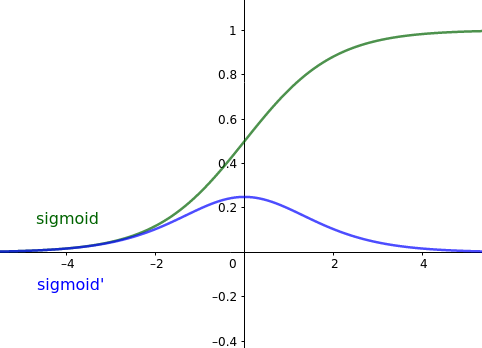
\includegraphics[width=0.4\linewidth]{img/fig_sig.png}
        \caption{sigmoid function and its derivative, x:y ratio 5:1 \label{fig:sigmoid}}
        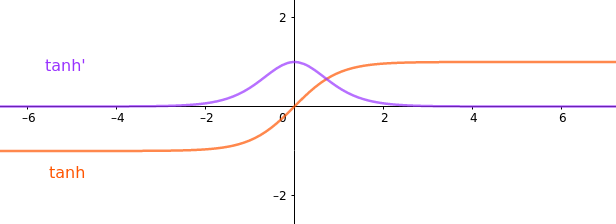
\includegraphics[width=0.6\linewidth]{img/fig_tanh.png}
        \caption{tanh function and its derivative, x:y ratio 1:1 \label{fig:tanh}}
        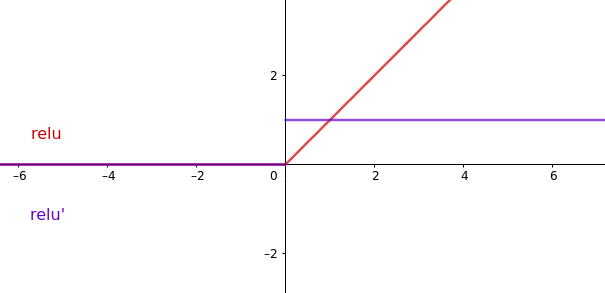
\includegraphics[width=0.6\linewidth]{img/fig_relu.png}
        \caption{ReLU function and its derivative, x:y ratio 1:1 \label{fig:relu}}
    \end{figure}
    
    \paragraph{b)}

    All functions (sigmoid: \Cref{fig:sigmoid}, tanh: \Cref{fig:tanh}, ReLU: \Cref{fig:relu}) are non-decreasing. Positive properties of sigmoid and tanh are that their derivatives are continuous and that they are bounded. Both sigmoid and ReLU are non-negative, though this is not an unfixable property of tanh, as it can be moved upward and squashed to also span $(0, 1)$. In fact tanh is just manipulated sigmoid. Tanh and sigmoid require quite demanding computations (can be approximated by precomputed lookup tables), while ReLU is only an \textit{if} statement.
    
    Sigmoid is more stretched along the x axis and therefore in comparison the gradient of tanh is more concentrated around the origin. This is also adjustable by just multiplying the argument by a parameter: $\alpha x$.
    
    Because of the almost constant derivative of ReLU, it could be difficult to navigate the function landscape with higher order approximation.
    
    \paragraph{c)}
    
    For binary classification, sigmoid or squashed tanh would make the most sense, because they would directly be able to output the probability of the first class and the probability of the other class as $1-p$ (property of them being bounded).
    
    For predicting multiple classes, both sigmoid and tanh would give the same argmax. This would not be the case for ReLU in case all of the feeding values would be $<0$. For multiclass prediction something like softmax (based on sigmoid) would be the most useful.
    
\end{solution}


\clearpage

\section*{Submission instructions}

\framebox{
	\begin{minipage}{\linewidth}
		The following instructions are mandatory. If you are not following them, tutors can
		decide to not correct your exercise.
	\end{minipage}
}

\begin{itemize}
    \item You have to submit the solutions of this assignment sheet as a team of 2-3 students.
    \item  Hand in a \textbf{single} PDF file with your solutions.
    \item Make sure to write the student teams ID and the name of each
    member of your team on your submission.
    \item Your assignment solution must be uploaded by only \textbf{one} of your team members to the course website.
    \item If you have any trouble with the submission, contact your tutor \textbf{before} the deadline.
\end{itemize}

\end{document}
